\documentclass[a4paper,11pt,twoside]{memoir}
\chapterstyle{veelo}

\usepackage{TUINFDA}

\usepackage{url}
\usepackage{hyperref}					% links in pdf
\usepackage{graphicx}            			% Figures
\usepackage{verbatim}            			% Code-Environment
\usepackage[lined,linesnumbered,algochapter]{algorithm2e} % Algorithm-Environment

\usepackage{pgf}					
\usepackage{tikz}					% tikz graphics
\usetikzlibrary{arrows,automata}

\usepackage{ngerman}
\usepackage[ngerman]{babel}
\usepackage{bibgerm,cite}       % Deutsche Bezeichnungen, Automatisches Zusammenfassen von Literaturstellen
\usepackage[ngerman]{varioref}  % Querverweise
% to use the german charset include cp850 for MS-DOS, ansinew for Windows and latin1 for Linux.
% \usepackage[latin1]{inputenc}

\thesistitle{Space \& Congruence Compression of Proofs}
%\thesissubtitle{Introducing $n$ quantified cuts into cut-free proofs in LK} % optional
\thesisdate{\today}

% all titles and designations have to be gender-related!
\thesisdegree{Diplomarbeit}{Master thesis}
\thesiscurriculum{European Master in Computational Logic}{European Master in Computational Logic} % your study
\thesisverfassung{Andreas Fellner, BSc} % Verfasser
\thesisauthor{Andreas Fellner, BSc} % your name
\thesisauthoraddress{Reihergraben 6a, 3400 Klosterneuburg} % your address
\thesismatrikelno{0825918} % your registration number

\thesisbetreins{Univ. Prof. Dr.phil. Alexander Leitsch}
\thesisbetrzwei{Bruno Woltzenlogel Paleo, MSc}

% define page numbering styles
\makepagestyle{numberCorner}
\makeevenfoot{numberCorner}{\thepage}{}{}
\makeoddfoot{numberCorner}{}{}{\thepage}

% define custom macros for specific formats or names
\newcommand{\uml}[1]{\texttt{#1}}
\newcommand{\cd}{\textsf{Class Diagram}}

\begin{document}

\captionnamefont{\bfseries}

%%%%%%%%%%%%%%%%%%%%%%%%%%%%%%%%%%%%%%%%%
%%%   FRONTMATTER    %%%%%%%%%%%%%%%%%%%%
%%%%%%%%%%%%%%%%%%%%%%%%%%%%%%%%%%%%%%%%%
\frontmatter
\pagenumbering{roman}

%%%%%%%%%%%%%%%%%%%%%%%%%%%%%%%%%%%%%%%%%
%%%   TITLEPAGES    %%%%%%%%%%%%%%%%%%%%%
%%%%%%%%%%%%%%%%%%%%%%%%%%%%%%%%%%%%%%%%%

% the german title page is required as first page
% $Id: titlepage.tex 1752 2010-03-20 11:07:02Z tkren $
%
% TU Wien - Faculty of Informatics
% thesis titlepage
%
% This titlepage is using the geometry package, see
% <http://www.ctan.org/macros/latex/contrib/geometry/geometry.pdf>
%
% For questions and comments send an email to
% Thomas Krennwallner <tkren@kr.tuwien.ac.at>
% or to Petra Brosch <brosch@big.tuwien.ac.at>
%

\selectlanguage{ngerman}

% setup page dimensions for titlepage
\newgeometry{left=2.4cm,right=2.4cm,bottom=2.5cm,top=2cm}

% force baselineskip and parindent
\newlength{\tmpbaselineskip}
\setlength{\tmpbaselineskip}{\baselineskip}
\setlength{\baselineskip}{13.6pt}
\newlength{\tmpparindent}
\setlength{\tmpparindent}{\parindent}
\setlength{\parindent}{17pt}

% first titlepage
\thispagestyle{tuinftitlepage}

%
% Kludge: for each titlepage set \pagenumbering to a different
% style. This is used to fix a problem with hyperref, because there
% are multiple "page 1" and hyperref hates that
%
\pagenumbering{Alph}

\begin{center}
{\ \vspace{3.4cm}}

\begin{minipage}[t][2.8cm][s]{\textwidth}%
\centering
\thesistitlefontHUGE\sffamily\bfseries\tuinfthesistitle\\
\bigskip
{\thesistitlefonthuge\sffamily\bfseries\tuinfthesissubtitle}
\end{minipage}

\vspace{1.3cm}

{\thesistitlefontLARGE\sffamily \tuinfthesistype}

\vspace{6mm}

%{\thesistitlefontlarge\sffamily zur Erlangung des akademischen Grades}

\vspace{6mm}

{\thesistitlefontLARGE\sffamily\bfseries \tuinfthesisdegree}

\vspace{6mm}

{\thesistitlefontlarge\sffamily im Rahmen des Studiums}

\vspace{6mm}

{\thesistitlefontLarge\sffamily\bfseries \tuinfthesiscurriculum}

\vspace{6.5mm}

{\thesistitlefontlarge\sffamily eingereicht von}

\vspace{6mm}

{\thesistitlefontLarge\sffamily\bfseries \tuinfthesisauthor}

\vspace{1.5mm}

{\thesistitlefontlarge\sffamily Matrikelnummer \tuinfthesismatrikelno} 

\vspace{1.4cm}

\vspace{0pt}\raggedright\thesistitlefontnormalsize\sffamily
\begin{minipage}[t][1.6cm][t]{\textwidth}%
  %
  an der

  Fakult\"{a}t f\"{u}r Informatik der Technischen Universit\"{a}t Wien
\end{minipage}

\begin{minipage}[t][4cm][t]{\textwidth}%
  \vspace{0pt}\raggedright\thesistitlefontnormalsize\sffamily
  %
  \begin{tabbing}%
	    \hspace{19mm} \= \hspace{66mm} \kill
	    \tuinfthesisbetreuung: \> \tuinfthesisbetreins\\
	    Mitwirkung: \> \tuinfthesisbetrzwei\\
	                \> \tuinfthesisbetrdrei
  \end{tabbing}
\end{minipage}

\begin{minipage}[t][1.5cm][t]{\textwidth}%
  \vspace{0pt}\sffamily\thesistitlefontnormalsize
  \begin{tabbing}%
    \hspace{45mm} \= \hspace{63mm} \= \hspace{51mm} \kill
    Wien, \tuinfthesisdate \> {\raggedright\rule{51mm}{0.5pt}} \> {\raggedright\rule{51mm}{0.5pt}} \\
    \> \begin{minipage}[t][0.5cm][t]{51mm}\centering (Unterschrift \tuinfthesisverfassung)\end{minipage}
    \> \begin{minipage}[t][0.5cm][t]{51mm}\centering (Unterschrift \tuinfthesisbetreuung)\end{minipage}
    \end{tabbing}
\end{minipage}

\end{center}

% we want an empty page right after first titlepage
\pagestyle{empty}
\cleardoublepage

% we're done with the titlepages, proceed with default pagenumbering
\pagenumbering{roman}

% restore baselineskip
\setlength{\baselineskip}{\tmpbaselineskip}
\setlength{\parindent}{\tmpparindent}

% back to normal geometry
\restoregeometry

\selectlanguage{english}

%%% Local Variables:
%%% TeX-PDF-mode: t
%%% TeX-debug-bad-boxes: t
%%% TeX-parse-self: t
%%% TeX-auto-save: t
%%% reftex-plug-into-AUCTeX: t
%%% End:


% an english translation may follow
% $Id: titlepage.tex 1752 2010-03-20 11:07:02Z tkren $
%
% TU Wien - Faculty of Informatics
% thesis titlepage
%
% This titlepage is using the geometry package, see
% <http://www.ctan.org/macros/latex/contrib/geometry/geometry.pdf>
%
% For questions and comments send an email to
% Thomas Krennwallner <tkren@kr.tuwien.ac.at>
% or to Petra Brosch <brosch@big.tuwien.ac.at>
%

% setup page dimensions for titlepage
\newgeometry{left=2.4cm,right=2.4cm,bottom=2.5cm,top=2cm}

% force baselineskip and parindent
%\newlength{\tmpbaselineskip}
%\setlength{\tmpbaselineskip}{\baselineskip}
%\setlength{\baselineskip}{13.6pt}
%\newlength{\tmpparindent}
%\setlength{\tmpparindent}{\parindent}
%\setlength{\parindent}{17pt}

% first titlepage
\thispagestyle{tuinftitlepage}

%
% Kludge: for each titlepage set \pagenumbering to a different
% style. This is used to fix a problem with hyperref, because there
% are multiple "page 1" and hyperref hates that
%
\pagenumbering{Roman}

\begin{center}
{\ \vspace{3.4cm}}

\begin{minipage}[t][2.8cm][s]{\textwidth}%
\centering
\thesistitlefontHUGE\sffamily\bfseries\tuinfthesistitle\\
\bigskip
{\thesistitlefonthuge\sffamily\bfseries\tuinfthesissubtitle}
\end{minipage}

\vspace{1.3cm}

%{\thesistitlefontLARGE\sffamily \tuinfthesistypeen}

\vspace{6mm}

%{\thesistitlefontlarge\sffamily submitted in partial fulfillment of the requirements for the degree of}

\vspace{6mm}

{\thesistitlefontLARGE\sffamily\bfseries \tuinfthesisdegreeen}

\vspace{6mm}

{\thesistitlefontlarge\sffamily in}

\vspace{6mm}

{\thesistitlefontLarge\sffamily\bfseries \tuinfthesiscurriculumen}

\vspace{6.5mm}

{\thesistitlefontlarge\sffamily by}

\vspace{6mm}

{\thesistitlefontLarge\sffamily\bfseries \tuinfthesisauthor}

\vspace{1.5mm}

{\thesistitlefontlarge\sffamily Registration Number \tuinfthesismatrikelno} 

\vspace{1.4cm}

\begin{minipage}[t][1.6cm][t]{\textwidth}%
  \vspace{0pt}\raggedright\thesistitlefontnormalsize\sffamily
  %
  to the Faculty of Informatics 

  at the Vienna University of Technology
\end{minipage}

\vspace{0pt}\raggedright\thesistitlefontnormalsize\sffamily
\begin{minipage}[t][4cm][t]{\textwidth}%
  \begin{tabbing}%
	    \hspace{19mm} \= \hspace{66mm} \kill
	    Advisor: \> \tuinfthesisbetreins\\
	    Assistance: \> \tuinfthesisbetrzwei\\
	                \> \tuinfthesisbetrdrei
     \end{tabbing}
\end{minipage}

\begin{minipage}[t][1.5cm][t]{\textwidth}%
  \vspace{0pt}\sffamily\thesistitlefontnormalsize
  \begin{tabbing}%
    \hspace{45mm} \= \hspace{63mm} \= \hspace{51mm} \kill
    Vienna, \tuinfthesisdate \> {\raggedright\rule{51mm}{0.5pt}} \> {\raggedright\rule{51mm}{0.5pt}} \\
    \> \begin{minipage}[t][0.5cm][t]{51mm}\centering (Signature of Author)\end{minipage}
    \> \begin{minipage}[t][0.5cm][t]{51mm}\centering (Signature of Advisor)\end{minipage}
    \end{tabbing}
\end{minipage}

\end{center}

% we want an empty page right after first titlepage
\pagestyle{empty}
\cleardoublepage

% we're done with the titlepages, proceed with default pagenumbering
\pagenumbering{roman}

% restore baselineskip
\setlength{\baselineskip}{\tmpbaselineskip}
\setlength{\parindent}{\tmpparindent}

% back to normal geometry
\restoregeometry


%%% Local Variables:
%%% TeX-PDF-mode: t
%%% TeX-debug-bad-boxes: t
%%% TeX-parse-self: t
%%% TeX-auto-save: t
%%% reftex-plug-into-AUCTeX: t
%%% End:
 % optional

%%%%%%%%%%%%%%%%%%%%%%%%%%%%%%%%%%%%%%%%%
%%%   ERKLAERUNG DER SELBSTAENDIGKEIT   %
%%%%%%%%%%%%%%%%%%%%%%%%%%%%%%%%%%%%%%%%%
\cleardoublepage
%\selectlanguage{ngerman}
%\chapter*{Erklärung zur Verfassung der Arbeit}

\tuinfthesisauthor\\
\tuinfthesisauthoraddress

\vspace*{1.2cm}

Hiermit erkläre ich, dass ich diese Arbeit selbständig verfasst habe, 
dass ich die verwendeten Quellen und Hilfsmittel vollständig angegeben 
habe und dass ich die Stellen der Arbeit - einschließlich Tabellen, 
Karten und Abbildungen -, die anderen Werken oder dem Internet im 
Wortlaut oder dem Sinn nach entnommen sind, auf jeden Fall unter Angabe 
der Quelle als Entlehnung kenntlich gemacht habe.\\

\vspace*{2cm}
\begin{tabbing}%
    \hspace{58mm} \= \hspace{28mm} \= \hspace{58mm} \kill
    {\raggedright\rule{58mm}{0.5pt}} \> \> {\raggedright\rule{58mm}{0.5pt}} \\
    \begin{minipage}[t][0.5cm][t]{58mm}
	\vspace{0pt}\sffamily\thesistitlefontnormalsize
	\centering (Ort, Datum)
    \end{minipage}
    \> \>
    \begin{minipage}[t][0.5cm][t]{58mm}
	\vspace{0pt}\sffamily\thesistitlefontnormalsize
	\centering (Unterschrift \tuinfthesisverfassung)
    \end{minipage}
\end{tabbing}


\selectlanguage{english}

%%%%%%%%%%%%%%%%%%%%%%%%%%%%%%%%%%%%%%%%%
%%%   ACKNOWLEDGEMENTS    %%%%%%%%%%%%%%%
%%%%%%%%%%%%%%%%%%%%%%%%%%%%%%%%%%%%%%%%%

% optional acknowledgements may be included in german or in english
%\chapter*{Danksagung}

Hier fügen Sie optional eine Danksagung ein.
 		% optional
%\chapter*{Acknowledgements}
\vspace*{\fill}

We would like to thank Robert Nieuwenhuis and Ashish Tiwari for answering questions about the short explanation decision problem and providing inspiration for the proof of its NP-completeness. Furthermore, we would like to thank Armin Biere for clarifying why resolution chains are not left-associative in the TraceCheck proof format. We also want to give credit to the website stackexchange.com, its children sites and all its contributors. Without this website and the seemingly endless source of information on very specific problems, this thesis and especially the implementation would not exist in this form.
\vspace*{\fill}	% optional

%%%%%%%%%%%%%%%%%%%%%%%%%%%%%%%%%%%%%%%%%
%%%   ABSTARCT    %%%%%%%%%%%%%%%%%%%%%%%
%%%%%%%%%%%%%%%%%%%%%%%%%%%%%%%%%%%%%%%%%

\chapter*{Abstract}

\section{Problem definition}

Proofs are the backbone of mathematics. 
They allow scientists to build theorems on top of another and thus discover new knowledge.
Proofs not only serve as stepping stones, they can also provide insight on the nature of the underlying problem.

Both statements are true for formal proofs as well.
Formal proofs allow system to trust the output of other systems and therefore they can safely be built on top of another. 
For example SAT-Solvers are used extensively in modern deductive systems \cite{Biere2009}. 
However, solvers may contain bugs. 
Therefore their output can not be trusted blindly.
A formal proof can assure the correctness of the output.
Formal proofs not only help in combining systems, they can also be used to obtain information about the underlying problem.
For example interpolants, which have important applications in Verification and Synthesis of programs \cite{McMill2005}, can be extracted from formal proofs \cite{Hofferek2013}.
From hereon, we mean formal proofs when speaking of proofs.

Typically problems that are tackled by automated systems are large. 
As a consequence proofs produced during the process are large.
So large that even for proof processing algorithms with low complexity, it is highly desirable to reduce the hardness of the input, while maintaining the quality of its conclusion.
Proof processing algorithms could be correctness checking, information extraction or proof manipulating techniques.
That is the problem that our work tackles.
We present methods to compress proofs, produced by SMT- or SAT- Solvers, w.r.t. two different measures.

The first measure is \emph{length}.
The length of a proof is the number of inferences.
For example the length of the resolution proof is the number of resolution applications.
The congruence reasoning part of SMT-proofs has often been found to be redundant.
Congruence reasoning derives equations of terms that are implied by a given set of input equations, 
using the four axioms \emph{reflexivity}, \emph{symmetry}, \emph{transitivity} and \emph{congruence}. 
It can be redundant in the sense that subsets of the input may suffice to derive certain equations.
%Such subsets correspond to proofs that are shorter, use less axioms and derive a stronger conclusion.
%Replacing subproofs corresponding to a set of equations, 

The second measure is \emph{space}.
Typically proofs are represented as directed acyclic graphs.
The space of a proof $p$ and a traversal order $\prec$ is the maximal number of nodes of that graph that have to be kept in memory at once, while processing $p$ following $\prec$.
The goal is to construct traversal orders for proofs with small space measures.

%The key insight towards space compression is, that when processing a proof, to compute the result of one node, only the results of a limited number of other nodes have to be in memory.
%The traversal order
%
%When traversing a proof following some traversal order, for every node there is a point, after which it will not be accessed.
%At this point the node can be dropped from memory.
%With the assumption that nodes are loaded into- and deleted from memory exactly once, it can not be dropped earlier.
%The traversal order 
%The goal is to construct traversal orders that induce small space measures.
%
%when operating on one node in general not all previously read nodes need to be in memory.
%every node at some point will be accessed the last time and can be dropped from memory after that point.
%at some point during the traversal every node will not be accessed anymore.

%To reduce the space measure of a proof, traversal orders can be constructed, that allow to drop nodes from memory early.

\section{State of the art}

The research field of proof complexity studies lower bounds of various measures of proofs in different proof calculi \cite{Arora2009,Beame1998a,Cook1979}. A typical questions of this fields intuitively is of the following kind. Given a proof calculus $\mathcal{C}$, find a sequence of theorems $(t_1,\ldots, t_n, \ldots)$ such that $\mathrm{length}(p(t_m)) \in \Omega(2^m)$, where $p(t)$ is a shortest proof of $t$ in $\mathcal{C}$.
%
 %and a problem $p \in \mathcal{P}$, where $\mathcal{P}$ is a class of problems, what is the worst case lower bound of some measure $m(.)$ of proofs, of all problems $p \in \mathcal{P}$ and their proofs in $\mathcal{C}$. % among all proofs in $\mathcal{C}$ of a problem $p$ or a problem class $\mathcal{P}$.
%
One classical result is the worst case exponential length of resolution refutations in the propositional resolution calculus \cite{Arora2009}.
Besides the classical length measure, space requirements of proofs have been studied \cite{Ben-Sasson2002,Esteban2001,Hopcroft1977,Nordstroem2013,Sethi1975} using pebbling games.
The problem of finding optimal strategies in the variant of the pebbling game that is most relevant to us is NP-complete \cite{Sethi1975}.

Our approach differs from this field of study, as we do not mean to prove new lower bounds for a class of problems or calculi, but to provide concrete algorithms to reduce measures of given proofs.

For Propositional Logic many length compression algorithms have been proposed \cite{Bar-Ilan2008,Bloem,Boudou2013,Cotton2010,Fontaine2011}. 
On the other hand, for First Order Logic Cut-Introduction has been studied \cite{Hetzl2012}, which is a form of proof compression. However, none of the approaches deal with the congruence reasoning of SMT-proofs. 
Congruence reasoning has been long studied and classical congruence closure algorithms are those of Nelson and Oppen \cite{Nelson1980}, Downey, Sethi and Tarjan \cite{Downey1980} and Shostak \cite{Shostak1978}.
More recently abstract congruence closure has been proposed \cite{Bachmair2000}, which replaces subterms with fresh constants to simplify the algorithms and increase performance.
Congruence closure algorithms producing explanations have been proposed by Pascal Fontaine \cite{Fontaine2004} and Nieuwenhuis-Oliveras \cite{Nieuwenhuis2007,Nieuwenhuis2005}.
The problem of deciding whether from a given set of equations, there is an explanation for one particular equation of size $k$ is believed to be NP-complete \cite{Nieuwenhuis2007,Nieuwenhuis2005}.
However, this result has not been proven yet.

Space compression of proofs is a young branch of proof compression and has not been studied extensively yet.
To the best of our knowledge neither an algorithm to compress proofs in space nor one to construct strategies in pebbling games has been proposed so far. 
The DRUP proof format \cite{Heule2013} is an extension of the well known RUP format, with the addition of deletion information. 
Deletion information indicates when nodes can be dropped from memory.
The format has been introduced to help cope with huge proofs produced by solvers. 
For example \cite{Konev2014} reports of a 13GB proof in the DRUP format for one case of the Erd\H{o}s Discrepancy Conjecture.
%Skeptik's native proof output format has already been enriched by optional deletion information.\\

\section{Methodology and approach}

We will propose algorithms for compressing proofs and show their complexity.
The algorithms will be implemented in the proof compression software Skeptik \cite{Boudou} in the programming language Scala.
We will evaluate the algorithms on a broad range of proofs produced by SAT- and SMT- Solvers to show the actual compression obtained.
The experiments will be carried out on the Vienna Scientific Cluster.
To remove redundancies in the congruence reasoning part of SMT- proofs, we will need two algorithms.

A congruence closure algorithm that is able to produce explanations in the form of proofs.
We will not use the ideas of abstract congruence closure, because we want to reduce the number of literals and therefore do not want to introduce new constants.
Even though the new constants can be removed from proofs, in our setting the algorithm will be applied many times to small instances and not the other way around. 
Therefore we think that the overhead of dealing with the extra constants is not worth the possible performance edge \cite{Bachmair2000} that abstract congruence closure can have when looking at single instances.
To obtain short proofs with short conclusions, we think that shortest path algorithms like the one of Dijkstra \cite{Dijkstra1959,Cormen1989} will be useful.

The second algorithm manipulates the proof itself.
It applies the congruence closure algorithm to the conclusions of subproofs reasoning about equality in order to find and remove redundancies.
The algorithm also fixes proof nodes with premises that have been changed by it earlier, similar to how it is described in \cite{Boudou2013}.
There can be a trade-off between the size of the proof and the size of its conclusion.
A shorter conclusion does not necessarily correspond to a shorter proof, if the original proof reuses some nodes many times.
However, shorter conclusions cause fewer inference steps further down the proof.
Intuitively shorter conclusions should always be better, but the relationship between proof- and conclusion size has to be investigated.


The algorithms to compress proofs in the space measure construct traversal orders using heuristics.
Traversal orders correspond to strategies in pebbling games.
The reason for the use of heuristics is the NP-completeness of finding optimal strategies in a variant of the pebble game \cite{Sethi1975} and the implied infeasibility of constructing the optimal strategy.
There will be two algorithms to construct traversal orders.
One operates on proofs in a Top-Down fashion, i.e. from the axioms towards the root, which corresponds to playing the pebbling game.
The other one operates on proofs in a Bottom-Up fashion, i.e. from the root towards the axioms, constructing orders by recursively queuing up premises.
The heuristics use characteristics of proof nodes, such as the number of children.

Theorems stating the complexity of our algorithms will have to be proven from scratch or adapted from earlier publications.

We want to show the NP-completeness of the shortest explanation problem.
To this end two things have to be done.
First we need to find an algorithm that, given an Oracle to make correct decisions, finds an explanation of $k$ or fewer equations in polynomial time.
Second we need to reduce another NP-complete problem to the shortest explanation problem.
The Palest Path Problem \cite{Tiwari} is one option for reduction, that has been foreseen to possibly be fruitful by the source of the claim in \cite{Nieuwenhuis2007,Nieuwenhuis2005}.

\section{Expected results}

We will enrich the field of proof compression by new algorithms.
It is hard to predict the compression achieved by the congruence reasoning algorithm.
Good propositional proof compression techniques usually achieve between 10\% and 20\% compression.
Such numbers would be nice to see for our method.
The space measure of a proof is always relative to a traversal order, therefore orders have to be compared to each other.
We hope to show that one method or heuristic is particularly better than the others.
The proof of NP-completeness of the shortest explanation problem is a gap in science, which we aim to fill.
\cleardoublepage
\selectlanguage{ngerman}
\chapter*{Kurzfassung}

Diese Arbeit befasst sich mit der Komprimierung von formalen Beweisen.
Formale Beweise sind von gro{\ss}er Bedeutung in der modernen Informatik.
Sie k\"onnen f\"ur den sicheren Austausch von deduktiven System verwendet werden.
Des Weiteren k\"onnen aus ihnen Informationen, wie etwa Interpolanten \cite{McMill2005}, extrahiert werden, welche zur L\"osung eines Problems beitragen \cite{Hofferek2013}.

Formale Beweise sind typischerweise sehr gro{\ss}, siehe etwa \cite{Konev2014} f\"ur einen 13GB Beweis eines Falles der Erd\H{o}s Discrepancy Conjecture.
Bei solchen Beweisgr\"o{\ss}en sto{\ss}en Computersysteme an ihre Grenzen und deswegen ist es erforderlich Beweise zu komprimieren.
Unsere Arbeit pr\"asentiert zwei Methoden zur Beweiskomprimierung.

Die erste Methode entfernt Redundanzen im Kongruenzteil von SMT-Beweisen.
Kongruenzbeweise schlie{\ss}en von einer Menge an Gleichungen auf neue Gleichungen mit der Vorraussetzung der vier Axiome: \emph{Reflexivit\"at}, \emph{Symmetrie}, \emph{Transitivit\"at} und \emph{Kongruenz}.
Beweise, die von SMT-Solvern erzeugt werden, schlie{\ss}en oft auf neue Gleichungen aus einer unn\"otig gro{\ss}en Menge.
Wir wollen kleinere Mengen finden, die f\"ur den Beweis der selben Aussage ausreichen und somit redundante Beweise durch k\"urzere ersetzen.
Au{\ss}erdem werden wir die NP-Vollst\"andigkeit des Problems der k\"urzesten Erkl\"arung einer Gleichung beweisen.

Die zweite Methode untersucht die Speicherplatzanforderungen von Beweisen.
Beim Bearbeiten von Beweisen muss nicht der gesamte Beweis zu jeder Zeit im Speicher gelagert werden.
Teilbeweise werden erst in den Speicher geladen, wenn sie ben\"otigt werden und werden wieder aus diesem entfernt, sobald sie nicht mehr ben\"otigt werden.
In welcher Ordnung die Teilbeweise geladen werden, ist essentiell f\"ur die maximale Speicherplatzanforderung.
Wir wollen Ordnungen mit niedrigen Speicherplatzanforderungen mit Hilfe von Heuristiken konstruieren.
\selectlanguage{english}

%%%%%%%%%%%%%%%%%%%%%%%%%%%%%%%%%%%%%%%%%
%%%   CONTENTS    %%%%%%%%%%%%%%%%%%%%%%%
%%%%%%%%%%%%%%%%%%%%%%%%%%%%%%%%%%%%%%%%%
% uncomment to set document language to german (results in "Inhaltsverzeichnis", "Kapitel", "Abbildung", etc. instead of "Contents", "Chapter", and "Figure"), otherwise the document's language is english
%\selectlanguage{ngerman}

\setcounter{tocdepth}{1}

\cleardoublepage
\pagestyle{numberCorner}
%\tableofcontents*

%%%%%%%%%%%%%%%%%%%%%%%%%%%%%%%%%%%%%%%%%
%%%   MAINMATTER    %%%%%%%%%%%%%%%%%%%%%
%%%%%%%%%%%%%%%%%%%%%%%%%%%%%%%%%%%%%%%%%

\mainmatter
\pagenumbering{arabic}
\pagestyle{numberCorner}

%%%%%%%%%%%%%%%%%%%%%%%%%%%%%%%%%%%%%%%%%
%\chapter{Introduction}
%\label{ch:intro}
%%%%%%%%%%%%%%%%%%%%%%%%%%%%%%%%%%%%%%%%%

%\section{Introduction}

\section{Problem definition}

Proofs are the backbone of mathematics. 
They allow scientists to build theorems on top of another and thus discover new knowledge.
Proofs not only serve as stepping stones, they can also provide insight on the nature of the underlying problem.

Both statements are true for formal proofs as well.
Formal proofs allow system to trust the output of other systems and therefore they can safely be built on top of another. 
For example SAT-Solvers are used extensively in modern deductive systems \cite{Biere2009}. 
However, solvers may contain bugs. 
Therefore their output can not be trusted blindly.
A formal proof can assure the correctness of the output.
Formal proofs not only help in combining systems, they can also be used to obtain information about the underlying problem.
For example interpolants, which have important applications in Verification and Synthesis of programs \cite{McMill2005}, can be extracted from formal proofs \cite{Hofferek2013}.
Since this work is concerned only with formal proofs, from hereon we mean formal proofs when speaking of proofs.

Typically problems that are tackled by automated systems are large. 
As a consequence proofs produced during the process are large.
So large that even for proof processing algorithms with low complexity, it is highly desirable to reduce the hardness of the input, while maintaining the quality of its conclusion.
Proof processing algorithms could be correctness checking, information extraction or proof manipulating techniques.
That is the problem that our work tackles.
We present methods to compress proofs, produced by SMT- or SAT- Solvers, w.r.t. two different measures.
Due to the enormous size of proofs our methods were constructed with the goal of low complexity in runtime.

The first measure is \emph{length}.
The length of a proof is the number of inferences.
For example the length of the resolution proof is the number of resolution applications.
The congruence reasoning part of SMT-proofs has often been found to be redundant.
Congruence reasoning derives equations of terms that are implied by a given set of input equations, 
using the four axioms \emph{reflexive}, \emph{symmetric}, \emph{transitive} and \emph{compatible}. 
It can be redundant in the sense that subsets of the input may suffice to derive certain equalities.
In chapter \ref{cha:congruence} we present resolution proofs extended by equality and a method to compress them using congruence closure.
Furthermore we show that finding the shortest set of input equations explaining a given equality is NP-complete.
This indicates that there is no efficient algorithm to compute the shortest explanation efficiently.
Therefore we propose ideas and methods to obtain short explanations, while not blowing up in complexity.
We present a new congruence closure algorithm, which uses curried terms and runs in the best known asymptotic runtime.
One benefit of our algorithm is the possibility to implement it using immutable data structures.
Such data structures are a central concept of functional programming languages.
Implementing proposed algorithms in a functional language, while maintaining the optimal runtime is far from being trivial.
Many algorithms, not only those for computing the congruence closure, rely on destructive calls, which implicitly modify many data structures with a single modification of one structure. 

The second measure is \emph{space}.
Typically proofs can be represented as directed acyclic graphs.
The space of a proof $p$ and a traversal order $\prec$ is the maximal number of nodes of that graph that have to be kept in memory at once, while processing $p$ following $\prec$.
The goal is to construct traversal orders for proofs with small space measures.
In chapter \ref{cha:pebbling} we present a method to compress resolution proofs in their space measure.
The problem of finding the shortest space measure of a proof can be reduced to finding the optional strategy in a pebbling game.
For this game it was proven that constructing the best strategy is NP-complete.
Just like for our length compression algorithm, we want an algorithm with a lower complexity.
Therefore we propose a heuristic method and arguments why our heuristics are reasonable.

Both methods have been implemented into the proof compression software Skeptik and were evaluated on a big number of proofs, produced by the SMT-Solver VeriT.
These proofs are mostly from the benchmarks of SMT-lib.
Additionally we evaluated on proofs that were used in \cite{Hofferek2013} to synthesize boolean functions by extracting an interpolant from a single proof.
The method in \cite{Hofferek2013} has high complexity and is therefore heavily dependent on the size of the proof.
Therefore compressing such proofs in reasonable time is a definite plus for their work and possible those of many others.


%%%%%%%%%%%%%%%%%%%%%%%%%%%%%%%%%%%%%%%%%
%\chapter{Typographic Design}
%\label{ch:typo}
%%%%%%%%%%%%%%%%%%%%%%%%%%%%%%%%%%%%%%%%%

%
For working with LaTeX you can take advantage of a variety of books and free introductions and tutorials on the internet. A competent contact point for LaTeX beginners is the LaTeX Wikibook, which is available under \url{http://en.wikibooks.org/wiki/LaTeX}. 

The following sections give examples of the most important LaTeX environments and commands.

\section{Tables}

Tables have to be realized with the help of the \textit{table} environment. Tables shall be sequentially numbered for each chapter and described in terms of a short caption (cf. Table~\ref{tab:diplomaseminar}).

\begin{table}[htb]
	\centering
	\begin{tabular}{|l|c|c|}
		\hline \textbf{Name} & \textbf{Date} & \textbf{Title} \\
		\hline
		\hline Mustermann Adam  & 18.5   & T1    \\
		\hline Musterfrau Eva  & 22.6   & T2    \\
		\hline
	\end{tabular}
	\caption{Seminar for Master Students}
	\label{tab:diplomaseminar}
\end{table}


\section{Figures}

Like tables, figures shall be sequentially numbered for each chapter and described in terms of a short caption). You could either produce your drawings directly inside Latex using PSTricks\footnote{\url{http://tug.org/PSTricks}}, Tikz\footnote{\url{http://sourceforge.net/projects/pgf}}, or any set of macros dedicated to your requirements (cf. Figure~\ref{fig:samplefigure_tikz}). Alternatively, you may include figures prepared in external tools (cf. Figure~\ref{fig:samplefigure_pdf}). Note, to ensure high quality printing, all figures must have at least 300 dpi.

\begin{figure}
	\centering
	\begin{tikzpicture}[->, auto, node distance=2.8cm, semithick]
	  \node[initial, state] (1)		 {$S_1$};
	  \node[state] 		(2) [right of=1] {$S_2$};
	
	  \path (1) edge [bend left]  node {0} (2)
		(1) edge [loop above] node {1} (1)
		(2) edge [bend left]  node {0} (1)
		(2) edge [loop above] node {1} (2);
	\end{tikzpicture}
	\caption{Sample figure}
	\label{fig:samplefigure_tikz}
\end{figure}

\begin{figure}[tb]
	\centering
	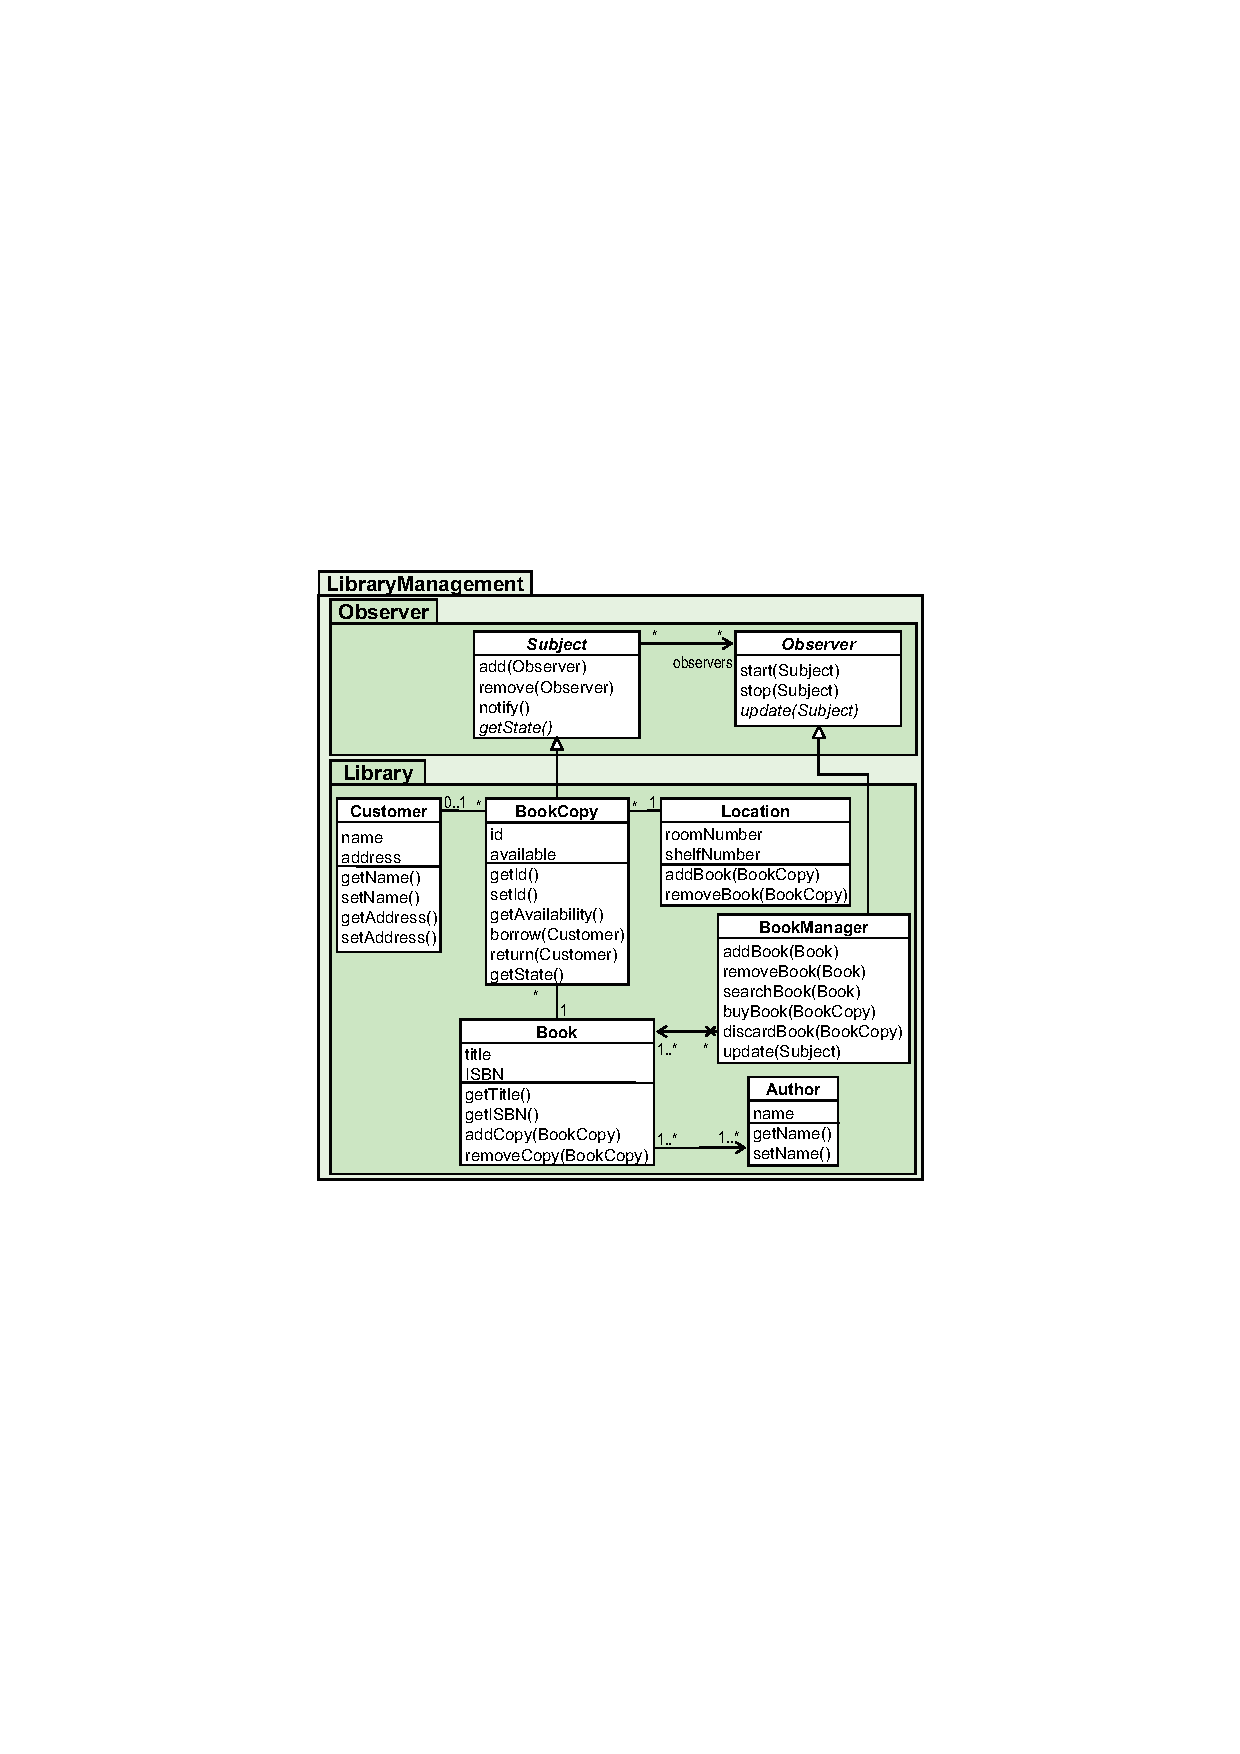
\includegraphics[width=0.7\textwidth]{figures/figure1}
	\caption{Sample figure}
	\label{fig:samplefigure_pdf}
\end{figure}


\section{Fonts}

When introducing important terms for the first time use \emph{emphasize}. For a consistent look and feel of proper names like {\cd} and {\uml{Observer}} pattern you may define macros in the main document \texttt{thesis.tex}.

\section{Code}

For short code fragments use the \textit{verbatim} environment.

\begin{verbatim}
//Start Program
System.out.println("Hello World!");
//End Program
\end{verbatim}

A much better alternative is the \textit{algorithm} environment (cf. Algorithm~\ref{alg:samplealgorithm}). This environment offers special formatting features for loops, operations and comments.

\begin{algorithm}[t]
\SetKwData{Left}{left}
\SetKwData{This}{this}
\SetKwData{Up}{up}
\SetKwFunction{Union}{Union}
\SetKwFunction{FindCompress}{FindCompress}
\SetKwInOut{Input}{input}
\SetKwInOut{Output}{output}

\Input{A bitmap $Im$ of size $w\times l$}
\Output{A partition of the bitmap}

\BlankLine

\emph{special treatment of the first line}\;
\For{$i\leftarrow 2$ \KwTo $l$}{
\emph{special treatment of the first element of line $i$}\;
\For{$j\leftarrow 2$ \KwTo $w$}{\label{forins}
\Left$\leftarrow$ \FindCompress{$Im[i,j-1]$}\;
\Up$\leftarrow$ \FindCompress{$Im[i-1,]$}\;
\This$\leftarrow$ \FindCompress{$Im[i,j]$}\;
\If(\tcp*[r]{O(\Left,\This)==1}){\Left compatible with \This}{\label{lt}
\lIf{\Left $<$ \This}{\Union{\Left,\This}}\;
\lElse{\Union{\This,\Left}\;}
}
\If(\tcp*[r]{O(\Up,\This)==1}){\Up compatible with \This}{\label{ut}
\lIf{\Up $<$ \This}{\Union{\Up,\This}}\;
\tcp{\This is put under \Up to keep tree as flat as possible}\label{cmt}
\lElse{\Union{\This,\Up}}\tcp*[r]{\This linked to \Up}\label{lelse}
}
}
\lForEach{element $e$ of the line $i$}{\FindCompress{p}}
}
\caption{Sample algorithm}\label{alg:samplealgorithm}
\end{algorithm}



%%%%%%%%%%%%%%%%%%%%%%%%%%%%%%%%%%%%%%%%%
%\chapter{Bibliographic Issues}
%\label{ch:bibliographic}
%%%%%%%%%%%%%%%%%%%%%%%%%%%%%%%%%%%%%%%%%

%\section{Literature Search}

Information on online libraries and literature search, e.g., interesting magazines, journals, conferences, and organizations may be found at \url{http://www.big.tuwien.ac.at/teaching/info.html}.

\section{BibTeX}

BibTeX should be used for referencing.

Blabla article1 \cite{hetzl2012towards}, laber laber article2 \cite{hetzl2014article}.

%%%%%%%%%%%%%%%%%%%%%%%%%%%%%%%%%%%%%%%%%
%%% BACKMATTER %%%%%%%%%%%%%%%%%%%%%%%%%%
%%%%%%%%%%%%%%%%%%%%%%%%%%%%%%%%%%%%%%%%%

\appendix

\bibliographystyle{plain}
\bibliography{references1}

\end{document}
